\chapter{Diseño e implementación} % Main chapter title

\label{Chapter3}

En este capítulo se describe la arquitectura global del prototipo, se detalla cada módulo hardware y software que lo compone, y se documentan las decisiones de implementación, los criterios de diseño y las pruebas preliminares realizadas. Se explican los flujos de datos entre el dispositivo de campo, el broker MQTT, el backend (API REST) y la interfaz web, y se resumen las consideraciones para el despliegue y el monitoreo post-implantación.


\section{Arquitectura del sistema}

La arquitectura propuesta separa de forma explícita el dispositivo de campo (contador + ESP32-C3 + SIM800L), el transporte de mensajes (broker MQTT) y los servicios de aplicación (API REST, persistencia y frontend). Esta separación facilita la interoperabilidad y permite desplegar la solución de forma local, remota o híbrida según las políticas institucionales


\subsection{Flujo de datos} 

\begin{itemize}

  \item Detección: el contador detecta un paso y envía una trama por RS-232 al ESP32-C3.

  \item Preprocesado en nodo: el firmware valida la trama, añade sello temporal y metadatos, y encola el evento en memoria (FIFO).

  \item Transmisión: cuando la conexión GPRS está disponible, el nodo publica el evento en el tópico MQTT \texttt{devices/\{device\_id\}/events}.
  
  \item Ingesta y persistencia: el broker Mosquitto entrega el mensaje al suscriptor backend, el servicio valida el payload y persiste el registro en la base de datos MySQL.
  
  \item Visualización/Control: la interfaz web consulta la API REST para datos históricos y recibe notificaciones en tiempo real.
  
  \item Emisión de comandos (desde UI): el operador genera un comando en la interfaz, la UI envía
  \texttt{POST /api/devices/\{id\}/commands} al backend, que crea un \texttt{cmd\_id} único y publica en \texttt{devices/\{device\_id\}/commands}.
  
  \item Recepción en nodo y entrega al contador: el ESP32-C3, suscrito a \texttt{devices/\{device\_id\}/commands}, recibe el comando, valida \texttt{cmd\_id} y lo envía al contador por RS-232, se aplica un timeout configurable por comando.
  
  \item Ejecución y ack: el contador ejecuta la orden y responde por RS-232, el firmware publica el ack/resultado en \texttt{devices/\{device\_id\}/status} con \texttt{cmd\_id} y \texttt{status} (\texttt{ok}, \texttt{failed}, \texttt{timeout}).

  \item Actualización en backend y UI: el suscriptor MQTT del backend recibe el ack, actualiza la tabla \texttt{commands} (campo \texttt{status}, \texttt{ack\_ts}) y notifica a la UI para que el operador vea el resultado.
\end{itemize}


\subsection{Descripción ampliada de bloques y responsabilidades}
\begin{itemize}

  \item {Bloque  Dispositivo de campo:} el nodo de campo integra el contador existente (salida RS-232), un microcontrolador ESP32-C3 y un módem GPRS SIM800L. El firmware, desarrollado sobre \texttt{ESP-IDF}, realiza las siguientes funciones: lectura continua de la trama serial, parsing tolerante a ruido, preprocesado (validación, normalización de campos y asignación de sello temporal UTC), encolamiento FIFO de eventos, gestión de reintentos y publicación MQTT cuando hay conectividad. Además, el nodo se suscribe a los tópicos de comandos y publica telemetría y acks. En el nodo se implementa persistencia mínima (registro de comandos pendientes y últimas N tramas) para recuperación tras reinicio.

  \item {Bloque Transporte (broker MQTT):} el broker actúa como bus de mensajes desacoplado. Se recomienda emplear \textit{Eclipse Mosquitto} en la etapa inicial y evaluar brokers gestionados para despliegues a mayor escala. El broker gestiona autenticación por credenciales, control de tópicos y, en producción, cifrado TLS. Se emplean tópicos jerárquicos por dispositivo para facilitar filtrado y autorización: 
\begin{itemize}
  \item \texttt{devices/\{device\_id\}/events}
  \item \texttt{devices/\{device\_id\}/commands} 
  \item \texttt{devices/\{device\_id\}/status}.
\end{itemize}


\item {Bloque Servidor central:} el servidor central reúne dos responsabilidades principales: 

\begin{itemize}  

\item  Componente suscriptor MQTT que valida, transforma y enruta mensajes hacia la lógica de negocio y la persistencia.

\item API REST que expone servicios de consulta, gestión y emisión de comandos. Esta separación permite que consumidores adicionales (por ejemplo, módulos analíticos) se suscriban al broker sin impactar la disponibilidad de la API. La persistencia se implementa en MySQL con un esquema relacional que soporta consultas por rango temporal, índices para rendimiento y auditoría de comandos.
 \end{itemize}

  \item {Bloque Cliente / visualización:} la interfaz web consume la API REST para consultas históricas y utiliza WebSocket o SSE para recibir eventos en tiempo real. Se eligió Ionic + Angular por su compatibilidad con entornos de escritorio y móviles y por facilitar un despliegue unificado. Las funciones principales del cliente son: visualización de eventos en tiempo real, consulta histórica filtrada, envío de comandos remotos con seguimiento de estado y panel de telemetría para mantenimiento preventivo.
\end{itemize}



La figura \ref{fig:diag_arquitectura} muestra el diagrama de arquitectura del sistema y el flujo de datos. 
El dispositivo de campo (contador + ESP32-C3 + SIM800L), broker MQTT ( Mosquitto),  servidor central (API REST en Node.js/Express + lógica de suscripción MQTT) y  cliente/visualización (interfaz web en Ionic/Angular).


\begin{figure}[htbp]
  \centering
  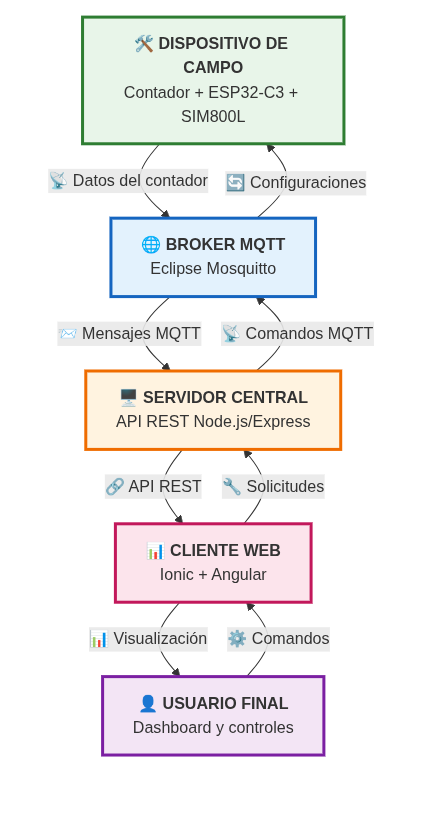
\includegraphics[width=0.4\linewidth]{./Figures/diagArq.png}
  \caption{Diagrama de arquitectura del sistema y el flujo de datos.}
  \label{fig:diag_arquitectura}
\end{figure}


\subsection{Decisiones de diseño clave}

\begin{itemize}

\item Separación broker/aplicación: permite cambiar broker o desplegar uno local sin tocar la lógica de negocio.

\item MQTT para mensajería ligera (QoS configurable) porque minimiza overhead en GPRS y facilita pub/sub.

\item API REST en Node.js/Express para exponer endpoints transaccionales y de gestión, centralizando autenticación y control de accesos.
\end{itemize}



\section{Detalle de módulos de hardware}
La implementación del prototipo requiere integrar componentes de hardware que permitan adaptar el sistema de detección de tránsito existente a un modelo de comunicación bidireccional. En esta sección se describen los módulos seleccionados, sus funciones principales, las interfaces involucradas y las consideraciones de integración.


\subsection{ESP32-C3 (unidad de control)}
El ESP32-C3 constituye el núcleo de procesamiento del nodo de campo. Se trata de un microcontrolador de bajo consumo con conectividad, elegido principalmente por su capacidad de cómputo, su soporte de entornos de desarrollo abiertos y la disponibilidad de bibliotecas optimizadas para protocolos de comunicación.

\begin{itemize}

\item Rol en la arquitectura: coordina la recepción de eventos desde el contador a través de RS-232, gestiona el encolamiento FIFO, controla la comunicación con el módem SIM800L mediante comandos AT y actúa como cliente MQTT.

\item Entorno de desarrollo: el firmware se desarrolló sobre ESP-IDF, el framework oficial de Espressif, que permite gestionar tareas concurrentes mediante FreeRTOS y facilita la integración de librerías de red y drivers UART.

\item Ventajas técnicas: bajo costo, consumo reducido, capacidad de ejecutar varias tareas en paralelo y soporte nativo para criptografía y seguridad en comunicaciones.

\item Consideraciones de diseño: se provee una correcta disipación térmica y  estabilidad de la alimentación, especialmente durante la transmisión de datos.

\end{itemize}

\subsection{Módulo GPRS SIM800L}

El módulo SIM800L implementa la conectividad celular GPRS, permitiendo la transmisión bidireccional de datos entre dispositivos remotos y servidor centralizado.


\begin{itemize}

\item Funciones principales: establecimiento de sesiones TCP/IP sobre GPRS, controlado por el ESP32-C3 mediante comandos AT. Soporta publicación y suscripción MQTT a través de sockets TCP persistentes.

\item Integración con ESP32-C3: la comunicación entre ambos se realiza mediante UART secundaria. El firmware implementa comandos de inicialización, registro en red, apertura de contexto y gestión de reconexiones.

\item Aspectos críticos: el SIM800L presenta picos de consumo que pueden superar los 2 A durante la transmisión, se  dispone de una fuente con suficiente margen y filtros adecuados para evitar reinicios inesperados.

\item Limitaciones: ancho de banda reducido (máximo teórico de 85,6 kbps en GPRS), lo que refuerza la decisión de emplear MQTT por su bajo overhead.

\end{itemize}


\subsection{Contador de tránsito y comunicación RS-232}

El sistema de conteo existente genera tramas con información de los eventos de paso de vehículos acumulados en un intervalo de tiempo (por defecto 1 hora). La comunicación con el ESP32-C3 se establece mediante interfaz RS-232, estándar ampliamente utilizado para transmisión serial de datos.

\begin{itemize}
\item Formato de trama:  el equipo incluye identificador de Dipositivo, timestamp local, valores de clasificación tránsito por carril.

\item Adaptación eléctrica: se utiliza un conversor de niveles (MAX232) para adaptar las señales RS-232 al rango TTL del microcontrolador.

\item Ventaja: la reutilización de la interfaz serial del contador evita modificar el sistema de detección existente, reduciendo costos de integración.


\end{itemize}


En la Figura \ref{fig:foto_dtec} se observa el contador de tránsito. Este dispositivo constituye la base del sistema de detección de eventos y se mantiene sin modificaciones en su lógica interna. 



\begin{figure}[htbp]
  \centering
  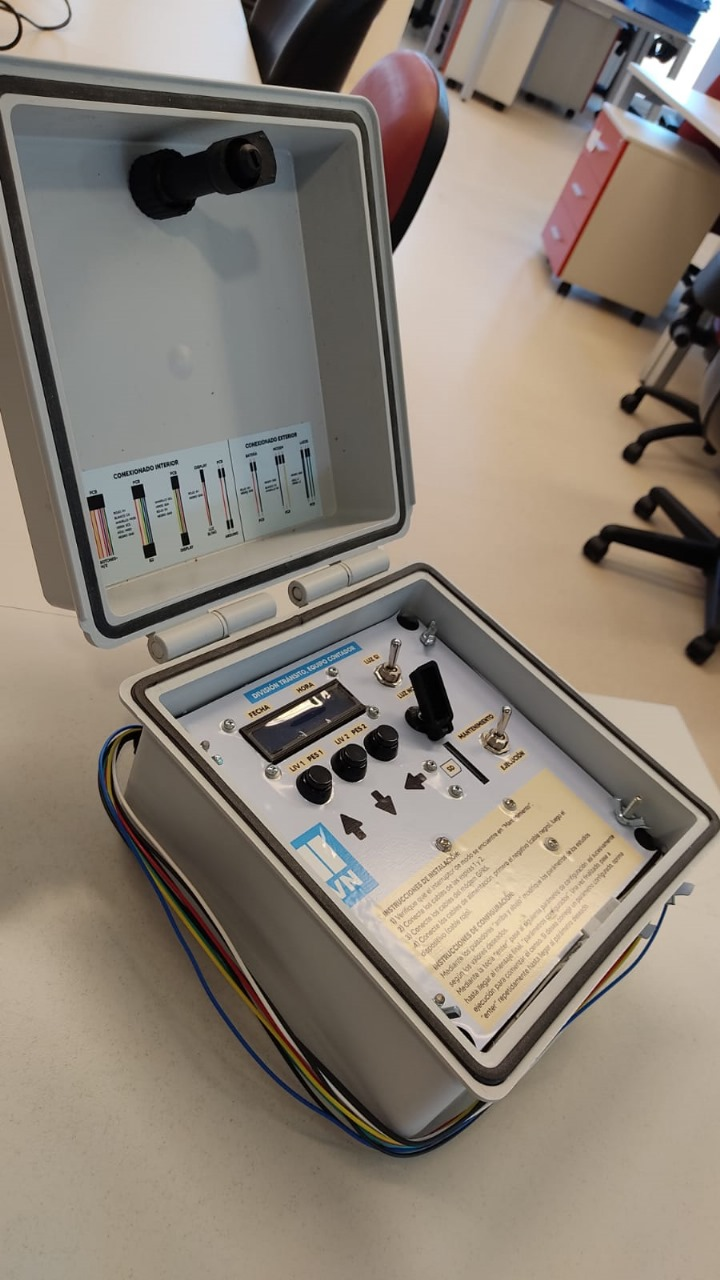
\includegraphics[width=0.5\linewidth]{./Figures/fotoDTEC.jpeg}
  \caption{Fotografia contador de tránsito DTEC \protect\footnotemark.}
  \label{fig:foto_dtec}
\end{figure}

\footnotetext{Imagen tomada de \url{http://transito.vialidad.gob.ar/}}

\subsection{Alimentación y montaje}

El nodo debe operar de manera confiable en condiciones de campo, por lo que la alimentación y el encapsulado son aspectos críticos.

\begin{itemize}
\item Fuente de alimentación: se empleó una fuente principal con batería interna recargable, diseñada para cubrir los picos de consumo del módulo SIM800L. La batería se recarga mediante un panel solar, lo que proporciona autonomía. Para estabilizar la entrega de energía se incorporó un módulo regulador de tensión que garantiza el nivel adecuado de voltaje para el módem. El circuito se complementó con capacitores dimensionados para absorber los picos de tensión del SIM800L durante la transmisión de datos, evitando caídas de voltaje que puedan reiniciar el sistema.

\item Carcasa y Gabinete: tanto el contador como el módulo de comunicación remota (ESP32-C3 y SIM800L) cuentan con su propia carcasa de protección y, adicionalmente, ambos se alojan en un gabinete cerrado con protección ambiental, diseñado para resistir humedad, polvo y vibraciones características de los entornos viales. El uso de un gabinete metálico contribuye también a la disipación térmica y a la reducción de interferencias electromagnéticas, asegurando la confiabilidad del sistema en condiciones de intemperie. 

\end{itemize}


